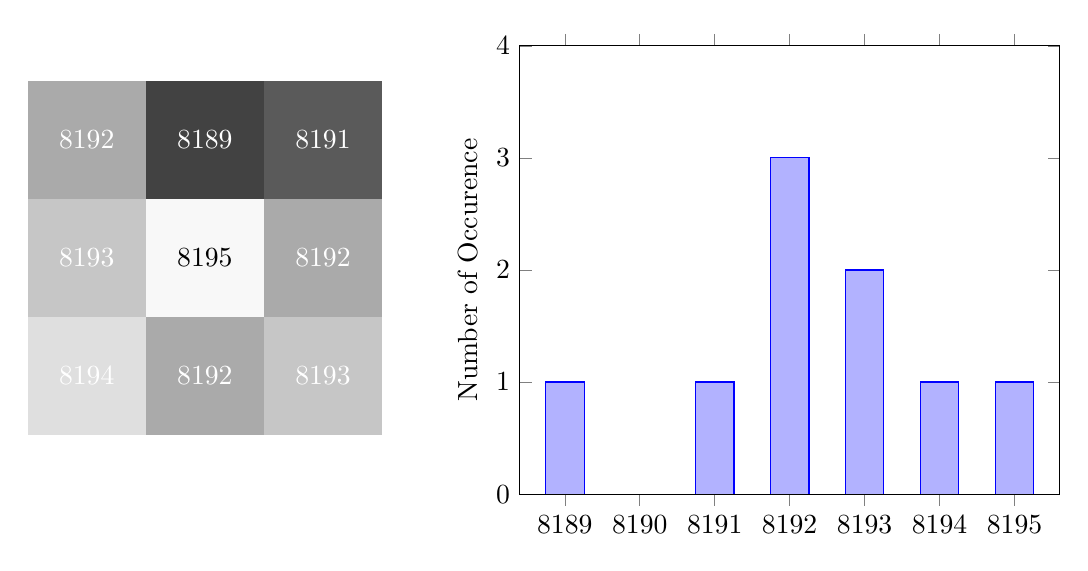
\begin{tikzpicture}
    \begin{scope}[xshift=-35mm]
        % upper row
        \node [rectangle, minimum size=15mm, fill={rgb,255:red,170; green,170; blue,170}](8192) at (1.5,4.5)   {\textcolor{white}{$8192$}};
        \node [rectangle, minimum size=15mm, fill={rgb,255:red,66; green,66; blue,66}](8189) at (3,4.5)     {\textcolor{white}{$8189$}};
        \node [rectangle, minimum size=15mm, fill={rgb,255:red,90; green,90; blue,90}](8191) at (4.5,4.5)   {\textcolor{white}{$8191$}};
        % mid row
        \node [rectangle, minimum size=15mm, fill={rgb,255:red,198; green,198; blue,198}](8193) at (1.5,3)     {\textcolor{white}{$8193$}};
        \node [rectangle, minimum size=15mm, fill={rgb,255:red,248; green,248; blue,248}](8195) at (3,3)       {\textcolor{black}{$8195$}};
        \node [rectangle, minimum size=15mm, fill={rgb,255:red,170; green,170; blue,170}](8192) at (4.5,3)     {\textcolor{white}{$8192$}};
        % lower row
        \node [rectangle, minimum size=15mm, fill={rgb,255:red,223; green,223; blue,223}](8194) at (1.5,1.5)   {\textcolor{white}{$8194$}};
        \node [rectangle, minimum size=15mm, fill={rgb,255:red,170; green,170; blue,170}](8192) at (3,1.5)     {\textcolor{white}{$8192$}};
        \node [rectangle, minimum size=15mm, fill={rgb,255:red,198; green,198; blue,198}](8193) at (4.5,1.5)   {\textcolor{white}{$8193$}};
    \end{scope}
    \begin{scope}[xshift=35mm]
        \begin{axis}[
            x tick label style={/pgf/number format/1000 sep=},
            ybar, bar width=14pt,
            ymin=0, ymax=4,
            ylabel = Number of Occurence,
            area style
        ]
    \addplot coordinates { (8189, 1) (8190, 0) (8191, 1) (8192, 3) (8193, 2) (8194, 1) (8195, 1) };
    \end{axis}
\end{scope}
\end{tikzpicture}
